\section{收敛方式}
\label{sec:rvconv-modes}

全章固定一个概率空间$(\Omega,\mathcal{F},\mathbb{P})$，在它上面讨论实随机变量$X_1,X_2,\dots$和一个候选极限$X$，它们都取有限实数值。要问的是$X_n$是否“趋于”$X$，所以把差
\[
 X_n-X
\]
当作共同的研究对象，称为第$n$项的误差。误差本身是$\Omega$上的函数，每个样本点$\omega$给出一个数$X_n(\omega)-X(\omega)$。

“误差趋于零”可以从三个角度提要求。逐样本：固定$\omega$，看数列$X_n(\omega)-X(\omega)$是否趋于零。逐事件：固定$n$和阈值$\varepsilon$，看误差超过$\varepsilon$这一事件的概率。逐平均：固定$n$，看误差绝对值的某次幂的期望。三个角度依次给出本节的三种收敛方式。

函数列的逐点、依测度与$L^{p}$收敛已经在一般测度空间上建立，可参考\BookChapterRef{chap:function-normed-spaces}{卷四第11章“赋范空间”}。本节不重复一般的定义和证明，而是在总质量为一的概率空间上解释每一种要求控制了什么、放过了什么。

\paragraph{贯穿全章的例子}
设$U_1,U_2,\dots$是相互独立的$\operatorname{Unif}(0,1)$随机变量，它们可以定义在同一个概率空间上（独立序列的构造见第~\ref{chap:probability-spaces}章），并记$U=U_1$。由它们构造下面几族随机变量，全章反复使用。第一族是累计最大值，第二族是独立示性变量，其中$p_n\in[0,1]$，$A_n=\{U_n<p_n\}$：
\[
 M_n=\max\{U_1,\dots,U_n\},\qquad \xi_n=\mathbf{1}_{A_n} .
\]
第三族是稀有大值：
\[
 Y_n=n\,\mathbf{1}_{\{U<1/n\}},\qquad Z_n=\sqrt{n}\,\mathbf{1}_{\{U<1/n\}} .
\]
第四族是移动区块$B_n$：第$k$层把$[0,1)$等分为$k$段，依次取各段的示性函数，具体写法见第~\ref{sec:rvconv-convergence-in-probability}小节。$M_n$的候选极限是常数$1$，其余几族的候选极限都是$0$。
$M_n$在三种意义下都收敛，其余几族各在某些意义下不收敛，用来检验各种收敛方式的边界。

\subsection{几乎必然收敛}
\label{sec:rvconv-almost-sure}

先把样本点$\omega$看成一次完整的观测记录。对累计最大值，$\omega$对应一串取值$U_1(\omega),U_2(\omega),\dots$，也就是无限次重复抽取的全部结果；记录一旦确定，$M_1(\omega),M_2(\omega),\dots$就是一列普通的数。图~\ref{fig:rvconv-max-paths}(a)画了五条这样的记录，每条记录上的误差$1-M_n(\omega)$都单调下降，并且迟早落到阈值$\varepsilon=0.1$以下。

\begin{BookInlineFigure}
 \centering
 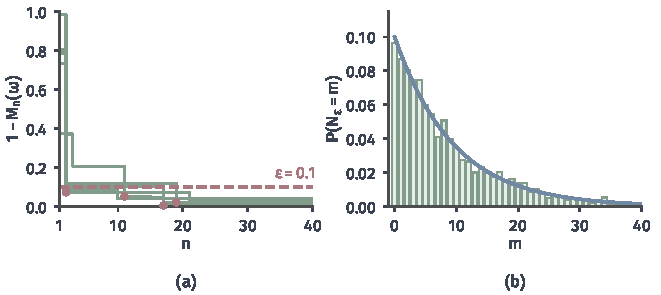
\includegraphics[width=112mm]{figures/07-probability/03-probability-limits/matplotlib/rvconv-max-paths/figure.pdf}
 \caption{累计最大值$M_n=\max\{U_1,\dots,U_n\}$的误差。(a)五条模拟记录上的$1-M_n(\omega)$（绿色台阶，种子$7$），红色虚线为阈值$\varepsilon=0.1$，红点标出误差最后一次降到阈值以下的位置。(b)最后一次超过阈值的序号$N_{\varepsilon}$：浅绿柱为$4000$条模拟记录的频率（种子$11$），蓝线为精确的质量$0.9^{m}\times0.1$。}
 \label{fig:rvconv-max-paths}
\end{BookInlineFigure}

\paragraph{例外的记录}
是不是每一条记录都如此？不是。若一条记录上所有$U_i(\omega)$都不超过$0.9$，比如每次都取到$0.5$，那么$M_n(\omega)\leq0.9$对一切$n$成立，误差永远不小于$0.1$。这样的记录是存在的，问题是它们一共有多大的概率。

$M_n(\omega)$随$n$递增且不超过$1$，所以它总收敛到$\sup_iU_i(\omega)$。它不收敛到$1$，当且仅当$\sup_iU_i(\omega)<1$，也就是存在正整数$k$，使所有$U_i(\omega)\leq1-1/k$。对固定的$k$和任意$n$，由独立性，
\[
 \mathbb{P}\bigl(U_i\leq1-\tfrac1k\text{ 对一切 }i\bigr)\leq\mathbb{P}\bigl(U_1\leq1-\tfrac1k,\dots,U_n\leq1-\tfrac1k\bigr)=\Bigl(1-\frac1k\Bigr)^{n}.
\]
右边随$n\to\infty$趋于零，左边与$n$无关，所以左边为零。再对$k=1,2,\dots$取并，可数个零概率事件的并仍是零概率事件，于是
\[
 \mathbb{P}\bigl(M_n\not\to1\bigr)=0 .
\]
例外的记录确实存在，但它们合在一起的概率为零。

\paragraph{定义}
这正是几乎必然收敛的含义：允许一个零概率的例外集合，在它之外，每条记录上的数列都收敛到目标。

\begin{definition}[几乎必然收敛]
\label{def:rvconv-almost-sure}
若
\begin{equation}
 \mathbb{P}\bigl(\{\omega:X_n(\omega)\to X(\omega)\}\bigr)=1 ,
 \label{eq:rvconv-almost-sure}
\end{equation}
称$X_n$\term{几乎必然收敛}（almost sure convergence）到$X$，记作$X_n\xrightarrow{\mathrm{a.s.}}X$。
\end{definition}

式~\eqref{eq:rvconv-almost-sure}里的集合是由可数次集合运算得到的事件，第~\ref{sec:rvconv-infinitely-often}小节会把它写出来。几乎必然收敛就是卷四所说的几乎处处收敛，只是测度换成了概率：例外集合$\{X_n\not\to X\}$是零概率事件。

\paragraph{同一个例外集}
定义里只有一个例外集合，它要容纳整列不收敛的所有记录。展开来说，存在零概率事件$N$，使得对每个$\omega\notin N$和每个$\varepsilon>0$，都有一个序号$N_{\varepsilon}(\omega)$，当$n>N_{\varepsilon}(\omega)$时
\[
 \lvert X_n(\omega)-X(\omega)\rvert\leq\varepsilon .
\]
这里$N_{\varepsilon}(\omega)$可以随记录改变，但一旦$\omega$在例外集之外，这一条记录从某项起就再也不会超差。

对累计最大值，$N_{\varepsilon}$可以取为误差最后一次超过$\varepsilon$的序号（从未超过时取$0$）。$1-M_n$随$n$递减，所以$N_{\varepsilon}\geq m$当且仅当$1-M_m>\varepsilon$，即前$m$次抽取都不超过$1-\varepsilon$。取$\varepsilon=0.1$，得到
\[
 \mathbb{P}(N_{\varepsilon}\geq m)=0.9^{m},\qquad
 \mathbb{P}(N_{\varepsilon}=m)=0.9^{m}\times0.1 .
\]
平均要等$\mathbb{E}[N_{\varepsilon}]=0.9/0.1=9$次以后误差才稳定在$0.1$以内，但个别记录要等几十次。图~\ref{fig:rvconv-max-paths}(b)的直方图和精确质量吻合：$N_{\varepsilon}$是一个处处有限的随机变量，而不是一个对所有记录都适用的常数。

\paragraph{与逐项保证的区别}
几乎必然收敛要和另一种看起来相近的说法分开。设对每个$n$，误差超标的概率都很小：
\[
 \mathbb{P}\bigl(\lvert X_n-X\rvert>\varepsilon\bigr)\leq\delta_n,\qquad \delta_n\to0 .
\]
这是对每一项分别作出的高概率保证，每一项都有自己的例外事件。这些例外事件随$n$改变，即使每一个都很小，它们也可能轮流覆盖整个$\Omega$，使得每条记录都无穷多次超标。下一小节的移动区块正是这种情形。

\paragraph{极限的唯一性}
几乎必然极限只能在零概率事件上有差别。若$X_n\xrightarrow{\mathrm{a.s.}}X$且$X_n\xrightarrow{\mathrm{a.s.}}X'$，两个收敛事件的概率都是$1$，它们的交的概率也是$1$。在交上，同一个数列的两个极限必须相等，所以
\[
 \mathbb{P}(X=X')=1 .
\]
反过来，把$X$在零概率事件上改值，几乎必然收敛不受影响。

\subsection{依概率收敛}
\label{sec:rvconv-convergence-in-probability}

几乎必然收敛要跟踪整条记录。很多时候我们只关心某个固定的样本量：抽了$n$次以后，误差大于$\varepsilon$的可能性有多大？这只涉及一个事件
\[
 \{\lvert X_n-X\rvert>\varepsilon\},
\]
称为第$n$项的超差事件。它是$\Omega$中的一个集合，大小用概率衡量。

对累计最大值，超差事件是
\[
 \{1-M_n>\varepsilon\}=\{U_1\leq1-\varepsilon,\dots,U_n\leq1-\varepsilon\},
\]
在$(U_1,\dots,U_n)$的单位立方体里是一个边长$1-\varepsilon$的小立方体。由独立性，它的概率是
\begin{equation}
 \mathbb{P}(1-M_n>\varepsilon)=(1-\varepsilon)^{n} .
 \label{eq:rvconv-max-tail}
\end{equation}
取$\varepsilon=0.1$，前三项是$0.9$、$0.81$、$0.729$，见图~\ref{fig:rvconv-error-event}；$n=10$时约为$0.3487$，$n=50$时约为$0.0052$。

\begin{BookInlineFigure}
 \centering
 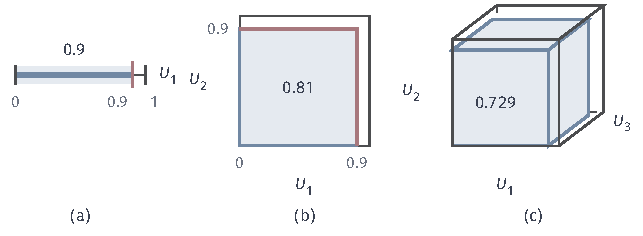
\includegraphics[width=109mm]{figures/07-probability/03-probability-limits/tikz/rvconv-error-event/figure.pdf}
 \caption{累计最大值的超差事件$\{1-M_n>0.1\}$。(a)$n=1$：线段$[0,0.9]$。(b)$n=2$：单位正方形中边长$0.9$的正方形，红线是事件的边界。(c)$n=3$：单位立方体中边长$0.9$的立方体。浅蓝区域的概率依次为$0.9$、$0.81$、$0.729$。}
 \label{fig:rvconv-error-event}
\end{BookInlineFigure}

\begin{definition}[依概率收敛]
\label{def:rvconv-in-probability}
若对每个$\varepsilon>0$，
\begin{equation}
 \lim_{n\to\infty}\mathbb{P}\bigl(\lvert X_n-X\rvert>\varepsilon\bigr)=0 ,
 \label{eq:rvconv-in-probability}
\end{equation}
称$X_n$\term{依概率收敛}（convergence in probability）到$X$，记作$X_n\xrightarrow{\mathbb{P}}X$。
\end{definition}

把“$>\varepsilon$”换成“$\geq\varepsilon$”得到同一个概念，因为两种事件互相夹住：
\[
 \{\lvert X_n-X\rvert>\varepsilon\}\subseteq\{\lvert X_n-X\rvert\geq\varepsilon\}\subseteq\{\lvert X_n-X\rvert>\varepsilon/2\} .
\]
由式~\eqref{eq:rvconv-max-tail}，$M_n\xrightarrow{\mathbb{P}}1$。依概率收敛就是卷四的依测度收敛，测度换成了概率。

\paragraph{移动区块}
依概率收敛只要求每一项的超差事件变小，并不要求它们停在同一个地方。下面的例子让超差事件在$\Omega$上来回移动。对$k=1,2,\dots$与$j=0,1,\dots,k-1$，令第$k$层第$j$段为$[j/k,(j+1)/k)$，按层从小到大、层内从左到右排成一列。第$n$项对应
\[
 n=\frac{k(k-1)}{2}+j+1,\qquad B_n=\mathbf{1}_{\{j/k\leq U<(j+1)/k\}} .
\]
前几项依次是$\mathbf{1}_{[0,1)}(U)$、$\mathbf{1}_{[0,1/2)}(U)$、$\mathbf{1}_{[1/2,1)}(U)$、$\mathbf{1}_{[0,1/3)}(U)$，等等。

对$0<\varepsilon<1$，第$n$项的超差事件就是$U$落在当前那一段，概率是段长$1/k$。$n$增大时层号$k$趋于无穷，所以
\[
 \mathbb{P}(\lvert B_n\rvert>\varepsilon)=\frac1k\to0,\qquad B_n\xrightarrow{\mathbb{P}}0 .
\]

但每一层的$k$段恰好铺满$[0,1)$，无论$U(\omega)$取什么值，每一层里都恰有一项等于$1$。所以对每一个$\omega$，数列$B_n(\omega)$中$1$出现无穷多次，$0$也出现无穷多次，它在任何一条记录上都不收敛。取$U(\omega)=0.37$，第$k$层里取值为$1$的是$j=\lfloor0.37k\rfloor$那一项，前几个序号是
\[
 n=1,\ 2,\ 5,\ 8,\ 12,\ 18,\ 24,\ 31,\ \dots
\]

\begin{BookInlineFigure}
 \centering
 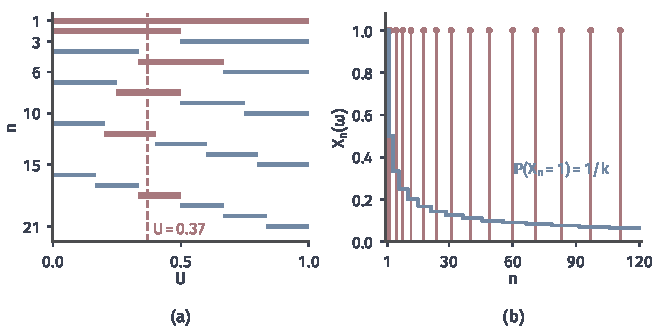
\includegraphics[width=112mm]{figures/07-probability/03-probability-limits/matplotlib/rvconv-blocks/figure.pdf}
 \caption{移动区块$B_n$。(a)前六层共$21$项：第$n$行的横条是$\{B_n=1\}$对应的$U$值区间，红色横条是被$U=0.37$穿过的那一项。(b)$U=0.37$这条记录上的$B_n(\omega)$，$n\leq120$：红色竖线标出取值为$1$的项；蓝色台阶是超差概率$\mathbb{P}(B_n=1)=1/k$。}
 \label{fig:rvconv-blocks}
\end{BookInlineFigure}

图~\ref{fig:rvconv-blocks}把两种读法放在一起。(a)中逐行看，每一行的横条越来越短，这是依概率收敛控制的量；沿红色虚线竖着看，就是一条记录，每一层都要碰到一个横条。(b)中蓝色台阶趋于零，红线却永不消失。大误差总会发生，只是发生在哪些记录上随$n$改变。

\paragraph{与几乎必然收敛对照}
两种收敛的差别在于控制的对象。依概率收敛逐次控制超差事件的大小，每个$n$单独检查；几乎必然收敛控制每条记录最终的行为，要求同一个$\omega$在某项之后再也不落入超差事件。前者是“在每一时刻，出问题的记录很少”，后者是“几乎每条记录，迟早不再出问题”。第~\ref{sec:rvconv-comparison}节证明后者推出前者，移动区块说明反过来不成立。

\paragraph{极限的唯一性与和的收敛}
依概率极限同样只在零概率事件上有差别。若$X_n\xrightarrow{\mathbb{P}}X$且$X_n\xrightarrow{\mathbb{P}}X'$，由三角不等式，$\lvert X-X'\rvert>2\varepsilon$时$\lvert X_n-X\rvert$与$\lvert X_n-X'\rvert$至少有一个大于$\varepsilon$，所以
\[
 \mathbb{P}\bigl(\lvert X-X'\rvert>2\varepsilon\bigr)\leq\mathbb{P}\bigl(\lvert X_n-X\rvert>\varepsilon\bigr)+\mathbb{P}\bigl(\lvert X_n-X'\rvert>\varepsilon\bigr).
\]
右边趋于零，左边与$n$无关，故为零。令$\varepsilon=1/k$并对$k$取可数并，得$\mathbb{P}(X\neq X')=0$。

同样的论证给出和的收敛：若$X_n\xrightarrow{\mathbb{P}}X$，$Y_n\xrightarrow{\mathbb{P}}Y$，则
\[
 \mathbb{P}\bigl(\lvert(X_n+Y_n)-(X+Y)\rvert>2\varepsilon\bigr)\leq\mathbb{P}\bigl(\lvert X_n-X\rvert>\varepsilon\bigr)+\mathbb{P}\bigl(\lvert Y_n-Y\rvert>\varepsilon\bigr)\to0 ,
\]
即$X_n+Y_n\xrightarrow{\mathbb{P}}X+Y$。两个超差事件各自很小，它们的并也很小，这种“并集上界”是处理依概率收敛的基本手段。

\subsection{\texorpdfstring{$L^{p}$}{Lp}收敛}
\label{sec:rvconv-lp}

超差概率只数大误差出现的机会，不管大误差有多大。另一种自然的要求是误差的平均大小趋于零。对$1\leq p<\infty$，误差绝对值的$p$次幂取期望，得到一个数$\mathbb{E}\bigl[\lvert X_n-X\rvert^{p}\bigr]$，大误差在其中按$p$次幂加权。

\begin{definition}[$L^{p}$收敛]
\label{def:rvconv-lp}
设$1\leq p<\infty$，$\mathbb{E}[\lvert X\rvert^{p}]<\infty$，且对每个$n$有$\mathbb{E}[\lvert X_n\rvert^{p}]<\infty$。若
\begin{equation}
 \lim_{n\to\infty}\mathbb{E}\bigl[\lvert X_n-X\rvert^{p}\bigr]=0 ,
 \label{eq:rvconv-lp}
\end{equation}
称$X_n$\term{$L^p$收敛}（convergence in $L^p$）到$X$，记作$X_n\xrightarrow{L^{p}}X$。
\end{definition}

矩有限的假设保证误差的$p$阶矩有意义。由$t\mapsto t^{p}$的凸性，对实数$a,b$有
\[
 \lvert a-b\rvert^{p}\leq2^{p-1}\bigl(\lvert a\rvert^{p}+\lvert b\rvert^{p}\bigr),
\]
所以$X_n$与$X$的$p$阶矩有限时，误差的$p$阶矩也有限。

把$p$阶矩开$p$次方，记
\[
 \lVert X\rVert_{p}=\bigl(\mathbb{E}[\lvert X\rvert^{p}]\bigr)^{1/p} ,
\]
它是卷四$L^{p}$范数在概率空间上的写法，$L^{p}$收敛就是$\lVert X_n-X\rVert_{p}\to0$。若同一列还$L^{p}$收敛到$X'$，由Minkowski不等式，
\[
 \lVert X-X'\rVert_{p}\leq\lVert X_n-X\rVert_{p}+\lVert X_n-X'\rVert_{p}\to0 ,
\]
左边与$n$无关，故为零，$X=X'$几乎必然。

\paragraph{平均绝对误差与均方误差}
$p=1$时，$\mathbb{E}[\lvert X_n-X\rvert]$是\emph{平均绝对误差}；$p=2$时，$\mathbb{E}[(X_n-X)^{2}]$是\emph{均方误差}，$L^{2}$收敛也称\term{均方收敛}（mean-square convergence）。目标是常数$c$时，均方误差可以拆成方差与偏差平方之和。在$X_n-c=(X_n-\mathbb{E}[X_n])+(\mathbb{E}[X_n]-c)$两边平方取期望，交叉项的期望为零，得到
\begin{equation}
 \mathbb{E}\bigl[(X_n-c)^{2}\bigr]=\operatorname{Var}(X_n)+\bigl(\mathbb{E}[X_n]-c\bigr)^{2} .
 \label{eq:rvconv-mse}
\end{equation}
所以$X_n\xrightarrow{L^{2}}c$当且仅当$\mathbb{E}[X_n]\to c$且$\operatorname{Var}(X_n)\to0$：均值要对准目标，波动要消失。

\paragraph{累计最大值的平均误差}
非负变量的矩可以由尾积分公式（第~\ref{chap:tail-probabilities}章）从生存函数算出：
\[
 \mathbb{E}[V^{p}]=\int_0^{\infty}p\,t^{p-1}\,\mathbb{P}(V>t)\,\mathrm{d}t .
\]
取$V=1-M_n$，它在$[0,1]$内取值，生存函数由式~\eqref{eq:rvconv-max-tail}给出。$p=1$时，
\[
 \mathbb{E}[1-M_n]=\int_0^{1}(1-t)^{n}\,\mathrm{d}t=\frac{1}{n+1} .
\]

$p=2$时，把$t=1-(1-t)$代入并分成两个积分，得到
\[
 \mathbb{E}\bigl[(1-M_n)^{2}\bigr]=2\int_0^{1}t(1-t)^{n}\,\mathrm{d}t=2\Bigl(\frac{1}{n+1}-\frac{1}{n+2}\Bigr)=\frac{2}{(n+1)(n+2)} .
\]
两者都趋于零，所以$M_n\xrightarrow{L^{1}}1$，$M_n\xrightarrow{L^{2}}1$。取$n=10$，平均绝对误差是$1/11\approx0.0909$，均方误差是$2/132\approx0.0152$。

用式~\eqref{eq:rvconv-mse}核对。偏差是$\mathbb{E}[M_{10}]-1=-1/11$，方差是均方误差减去偏差平方：
\[
 \operatorname{Var}(M_{10})=\frac{2}{132}-\frac{1}{121}\approx0.01515-0.00826=0.00689 .
\]
两部分大小相当：$M_n$总是低估$1$，平均低估$1/(n+1)$，同时围绕自己的均值波动。

\paragraph{稀有大值}
$L^{p}$收敛对大误差特别敏感。看$Z_n=\sqrt{n}\,\mathbf{1}_{\{U<1/n\}}$：它以概率$1/n$取$\sqrt n$，其余时候取$0$，所以
\begin{equation}
 \mathbb{E}\bigl[\lvert Z_n\rvert^{p}\bigr]=n^{p/2}\cdot\frac1n=n^{p/2-1} .
 \label{eq:rvconv-spike-moments}
\end{equation}
$p=1$时这是$n^{-1/2}\to0$，$p=2$时恒为$1$，$p=3$时是$n^{1/2}\to\infty$。同一列变量$L^{1}$收敛到$0$，却不$L^{2}$收敛。

把高度换成$n$，$Y_n=n\,\mathbf{1}_{\{U<1/n\}}$的平均绝对误差恒为$\mathbb{E}[Y_n]=1$，连$L^{1}$收敛也不成立。另一方面，$Y_n$与$Z_n$都在$U\geq1/n$时为零；对任何$U(\omega)>0$，$n>1/U(\omega)$以后两者都等于$0$，而$\mathbb{P}(U=0)=0$，所以它们都几乎必然收敛到$0$。超差概率是$1/n$，它们也依概率收敛到$0$。误差发生得越来越少，但每次发生时越来越大，平均误差能否消失取决于“少”与“大”谁占上风，而$p$越大，大误差的分量越重。

移动区块则相反：误差只取$0$和$1$，没有大值，$\mathbb{E}[\lvert B_n\rvert^{p}]=1/k\to0$，所以它在每个$L^{p}$中收敛到$0$，尽管在任何一条记录上都不收敛。

\paragraph{随机向量}
以上三种收敛对随机向量$\bm{X}_n,\bm{X}\in\mathbb{R}^{d}$同样适用，只需把$\lvert X_n-X\rvert$换成欧氏范数$\lVert\bm{X}_n-\bm{X}\rVert_2$。由于对每个分量$i$都有
\[
 \lvert x_i\rvert\leq\lVert\bm{x}\rVert_2\leq\lvert x_1\rvert+\dots+\lvert x_d\rvert ,
\]
向量的每一种收敛都等价于各个分量的同种收敛。维数固定时，只需研究实随机变量。
